\section{Buck-converter\label{Buck-C}}

The task of a buck converter is to be changing the input voltage to a lower output voltage. The components, which are needed, are a DC-source for input voltage, a switch contained a diode and a MOSFET, an inductor, a capacitor and a resistor for the load. The equivalent diagram in figure \ref{Buck-converter} illustrated a buck-converter.

\begin{figure}[htbp]
	\begin{center}
		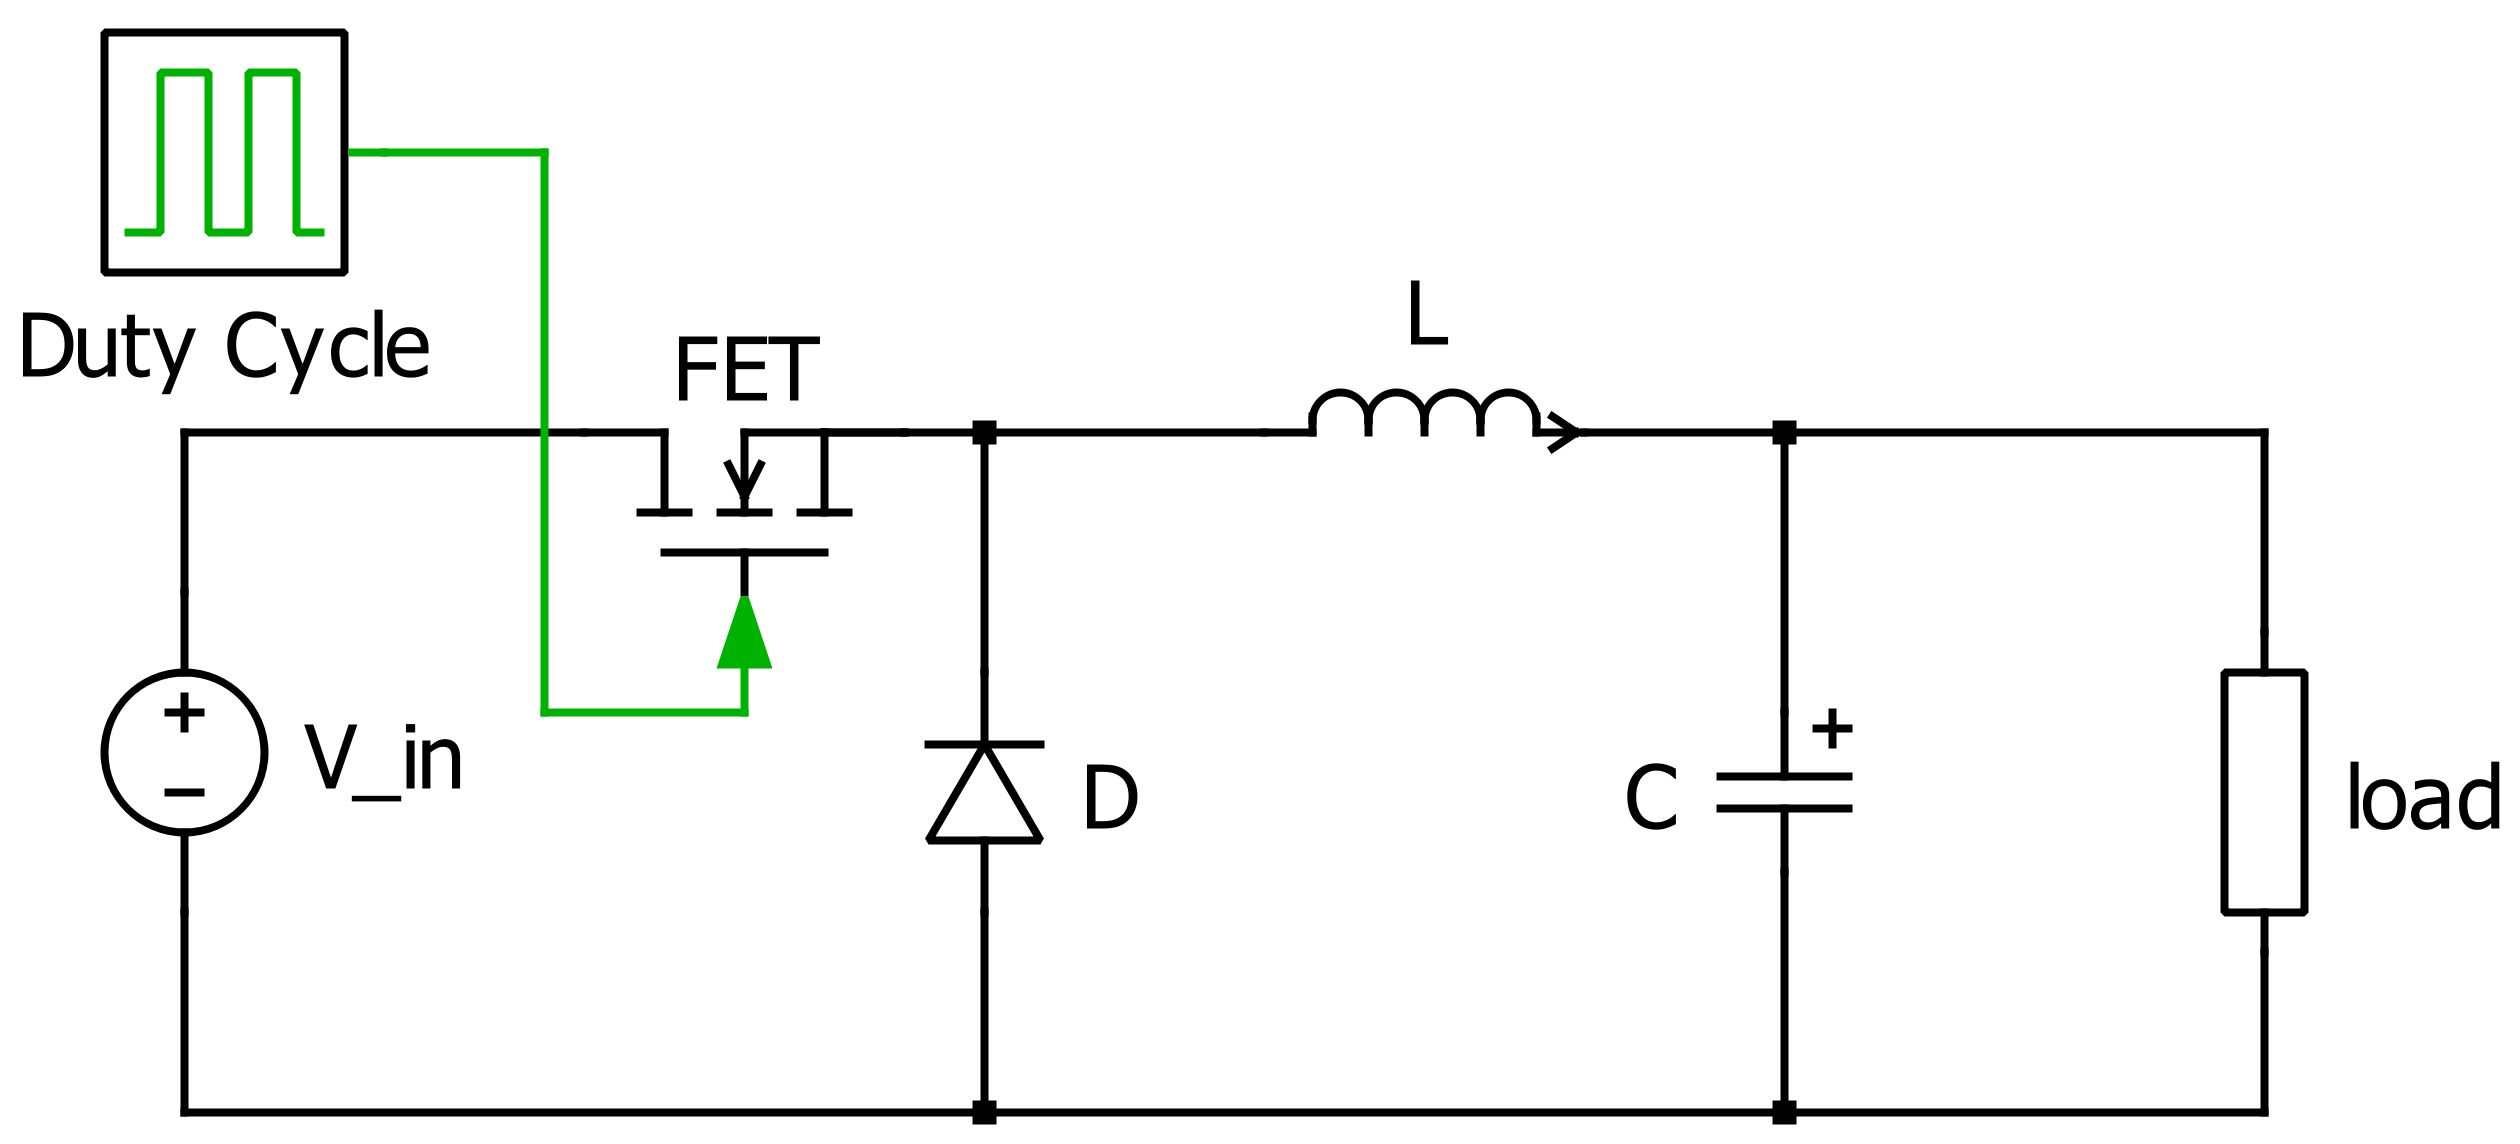
\includegraphics[width=0.7\textwidth]{../Pictures/Buck-converter}
		\caption{Buck-converter.}
		\label{Buck-converter}
	\end{center}	
\end{figure}

A buck-converter perform in two operating modes. In both operating modes have been an approach that the converter is in steady state and because of that, the average of a value is constant. Therefore, we can assume a DC-voltage at the load. At the case, that the MOSFET conducts current, the diode will be closed and the voltage drops at the inductor. Thus,  you can measure a lower voltage at the load. Besides that, the capacitor is loaded energy and the inductor is loaded current. If the MOSFET doesn't conduct current, the inductor will work as a current source and feeds the closed circuit with current. The capacitor is discharging and supplied the load.

The advantage for using a buck converter is that the structure is very simple and you need one power switch. The size for the component is small and the cost for this are low. Furthermore, the buck converter has a high efficiency of over 90 %.

So we come to the disadvantages from a buck converter. The transient response is slow for changes. 


\section{Boost-converter\label{Boost-C}}

A boost converter produces a higher output voltage in comparison to the input voltage. The circuit exists of a switch, which obtains a diode and a MOSFET, an inductor, a conductor, a resistor as a load and a DC-Source for the input voltage.Figure \ref{Boost-converter} shows an equivalent circuit diagram with the above-called components. Also for the boost-converter apply the steady state.

\begin{figure}[htbp]
	\begin{center}
		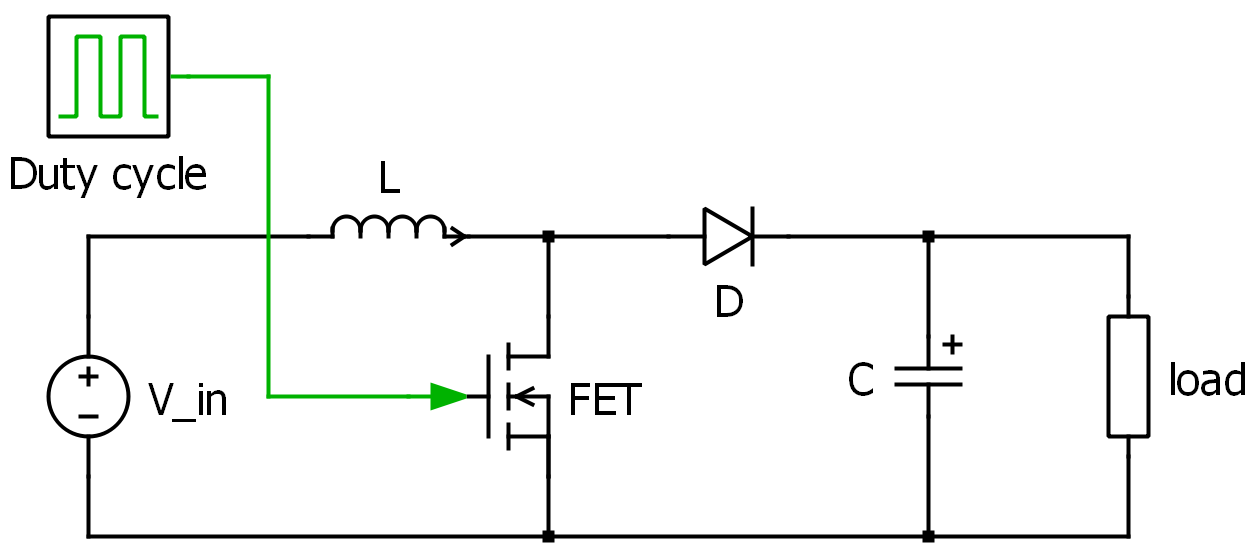
\includegraphics[width=0.7\textwidth]{../Pictures/Boost-converter}
		\caption{Boost-converter.}
		\label{Boost-converter}
	\end{center}	
\end{figure}

If the switch is closed, the inductor will increase the current in the circuit and it stored energy in itself. If the MOSFET is on, the current will flow only through the inductor because the diode is closed. The inductor increases the current in the circuit. Meanwhile, the capacitor releases the stored energy to the load. Thus, the output voltage decreases slowly. In the other case, when the MOSFET doesn’t conduct, the diode lets the current flow through the right side of the circuit. The current in the whole circuit decrease because of the higher impedance in this mode and the polarity of the inductor inverses itself. Therefore, the inductor performs as a source and the output voltage will be higher than the input voltage. Furthermore, the capacitor is charged.

An advantage for a boost converter is that it can raise the output voltage without help from a transformer. 
The size for the inductor and capacitor will have to be large, if you want a output without ripple. Furthermore changing the output voltage to big difference potential in the duty cycle can destroy components. If the switch is opened, current with a high peak flows through the diode and it can destroy it.
%%
